
\documentclass[twoside]{article}
\setlength{\oddsidemargin}{0.25 in}
\setlength{\evensidemargin}{-0.25 in}
\setlength{\topmargin}{-0.6 in}
\setlength{\textwidth}{6.5 in}
\setlength{\textheight}{8.5 in}
\setlength{\headsep}{0.75 in}
\setlength{\parindent}{0 in}
\setlength{\parskip}{0.1 in}

\usepackage{graphicx}
\usepackage{url}

%
% The following commands sets up the lecnum (lecture number)
% counter and make various numbering schemes work relative
% to the lecture number.
%
\newcounter{lecnum}
\renewcommand{\thepage}{\thelecnum-\arabic{page}}
\renewcommand{\thesection}{\thelecnum.\arabic{section}}
\renewcommand{\theequation}{\thelecnum.\arabic{equation}}
\renewcommand{\thefigure}{\thelecnum.\arabic{figure}}
\renewcommand{\thetable}{\thelecnum.\arabic{table}}
\newcommand{\dnl}{\mbox{}\par}

%
% The following macro is used to generate the header.
%
\newcommand{\lecture}[4]{
  \pagestyle{myheadings}
  \thispagestyle{plain}
  \newpage
  \setcounter{lecnum}{#1}
  \setcounter{page}{1}
  \noindent
  \begin{center}
  \framebox{
     \vbox{\vspace{2mm}
   \hbox to 6.28in { {\bf COMPSCI~590S~~~Systems for Data Science
                       \hfill Fall 2017} }
      \vspace{4mm}
      \hbox to 6.28in { {\Large \hfill Lecture #1: #2  \hfill} }
      \vspace{2mm}
      \hbox to 6.28in { {\it Lecturer: #3 \hfill Scribe(s): #4} }
     \vspace{2mm}}
  }
  \end{center}
  \markboth{Lecture {#1}: #2}{Lecture {#1}: #2}
  \vspace*{4mm}
}

%
% Convention for citations is authors' initials followed by the year.
% For example, to cite a paper by Leighton and Maggs you would type
% \cite{LM89}, and to cite a paper by Strassen you would type \cite{S69}.
% (To avoid bibliography problems, for now we redefine the \cite command.)
%
\renewcommand{\cite}[1]{[#1]}

% \input{epsf}

%Use this command for a figure; it puts a figure in wherever you want it.
%usage: \fig{NUMBER}{FIGURE-SIZE}{CAPTION}{FILENAME}
\newcommand{\fig}[4]{
           \vspace{0.2 in}
           \setlength{\epsfxsize}{#2}
           \centerline{\epsfbox{#4}}
           \begin{center}
           Figure \thelecnum.#1:~#3
           \end{center}
   }

% Use these for theorems, lemmas, proofs, etc.
\newtheorem{theorem}{Theorem}[lecnum]
\newtheorem{lemma}[theorem]{Lemma}
\newtheorem{proposition}[theorem]{Proposition}
\newtheorem{claim}[theorem]{Claim}
\newtheorem{corollary}[theorem]{Corollary}
\newtheorem{definition}[theorem]{Definition}
\newenvironment{proof}{{\bf Proof:}}{\hfill\rule{2mm}{2mm}}

% Some useful equation alignment commands, borrowed from TeX
\makeatletter
\def\eqalign#1{\,\vcenter{\openup\jot\m@th
 \ialign{\strut\hfil$\displaystyle{##}$&$\displaystyle{{}##}$\hfil
     \crcr#1\crcr}}\,}
\def\eqalignno#1{\displ@y \tabskip\@centering
 \halign to\displaywidth{\hfil$\displaystyle{##}$\tabskip\z@skip
   &$\displaystyle{{}##}$\hfil\tabskip\@centering
   &\llap{$##$}\tabskip\z@skip\crcr
   #1\crcr}}
\def\leqalignno#1{\displ@y \tabskip\@centering
 \halign to\displaywidth{\hfil$\displaystyle{##}$\tabskip\z@skip
   &$\displaystyle{{}##}$\hfil\tabskip\@centering
   &\kern-\displaywidth\rlap{$##$}\tabskip\displaywidth\crcr
   #1\crcr}}
\makeatother

% **** IF YOU WANT TO DEFINE ADDITIONAL MACROS FOR YOURSELF, PUT THEM HERE:

\usepackage{listings}
\usepackage{color}

\definecolor{dkgreen}{rgb}{0,0.6,0}
\definecolor{gray}{rgb}{0.5,0.5,0.5}
\definecolor{mauve}{rgb}{0.58,0,0.82}

\lstset{frame=tb,
  language=Java,
  aboveskip=3mm,
  belowskip=3mm,
  showstringspaces=false,
  columns=flexible,
  basicstyle={\small\ttfamily},
  numbers=none,
  numberstyle=\tiny\color{gray},
  keywordstyle=\color{blue},
  commentstyle=\color{dkgreen},
  stringstyle=\color{mauve},
  breaklines=true,
  breakatwhitespace=true,
  tabsize=3
}

% Some general latex examples and examples making use of the
% macros follow.

\begin{document}

%FILL IN THE RIGHT INFO.
%\lecture{**LECTURE-NUMBER**}{**DATE**}{**LECTURER**}{**SCRIBE**}
\lecture{5}{Databases vs. MapReduce}{Emery Berger}{Aishwarya Turuvekere, Suraj Subraveti}

\section{Review of MapReduce and Database performance}
We reviewed papers that dealt with MapReduce, a fault tolerant programming paradigm for processing and creating huge datasets, built by Google. There was also another paper that described how the growing popularity of MapReduce based systems didn't necessarily mean that databases have become irrelevant. Both papers discussed their pros and cons, and suggested ways in which a hybrid system could leverage the advantages of both paradigms.
\subsection{Pre-database systems}
Before databases became a popular way for querying for data, it was stored as files on disk, and these had "records" of fixed length. To access anything, one had to iterate through this file using a cursor. That would involve writing code like this:
\begin{lstlisting}
cursor c = file.begin();
while(cursor!=file.end()){
    String s = c.getNextRecord();
    //do something with the record
    c.moveToNextRecord();
}
\end{lstlisting}
For more complex operations, sorting the file on a particular field could be useful. For files that do not fit into the memory, some external sorting algorithm is required. This means that you would load chunks of the file into memory, and sort them, and merge these chunks until the file would be completely sorted, which is maybe okay if the data in the file is read only, but bad if there need to be updates performed, because one would need to sort the file each time something is updated. This costs a lot of I/O operations.

\subsection{Databases}
There are row and column store databases. Databases operate in an ACID fashion (Atomicity, Consistency, Isolation, Durability) via transactions. Prior to SQL (Structured Query Language) was QUEL, which became SEQUEL, then SQL. SQL is a declarative language. This means that the programmer states what they want done, and behind the scenes the interpreter determines the step(s) to complete the task(s).
An example database with an imperative program instead of a declaritive query.\\
\begin{tabular}{c|c|c}
Income & Name & Age\\
\hline
23000 & Brown & 29 \\
 & & .. \\
 & & .. \\
 \hline
\end{tabular}
\\
\begin{lstlisting}
it = db.begin();
count = 0;
for( , it!db.end(); it++)
    {
        if(it.getField("income")>100000){
            count++;
        }
    }
\end{lstlisting}

A query in a declaritive language will have a much different set of steps. For a query such as an insert, one might use a binary search to locate the correct location to insert a new record based on a given index or set of indices. This index could be represented as a B-tree. The result of these differences is that for tasks commonly done with a declaritive language like SQL, the imperative version of that program is much harder to write in a performative manner. Imperative languages can't hide details like index creation. C\# and link use SQL-like code in an imperative language to avoid the problems of imperative code.\\
There is a standard for SQL, but each vendor has its own dialect of SQL. A SQL query will be of the general form:\\
\begin{lstlisting}
SELECT...
FROM...
WHERE...
\end{lstlisting}
An example query would be:
\begin{lstlisting}
SELECT (*)
FROM employee 
WHERE employee.income > 100000;
\end{lstlisting}

When using SQL, one must be very explicit about the contents of the database. For this, the user specifies the content type of each column of each table in each database in what is known as a schema. The schema must be made prior to the creation of the table. \\
DBMS's don't have the advantage when it comes to semi-structured data. XML is a disaster. It encompasses HTML, but HTML on the web is rarely HTML compliant. Browsers tend to interpret HTML. MR can be a better fit in these cases because it is difficult to put webpages into databases.



\subsection{Row based vs Column based}
A database may be row based or column based. This is an implementation detail about the orientation of the data as it is stored on disk. A row based database will store an entire row contiguously on disk. This leads to a performance advantage when pulling an entire record or set of records from disk, as well as being straightforward to implement. This is also an advantage when distributing the database across multiple machines.\\
A column based database stores an entire column contiguously on disk. When accessing or appending entire rows, this will be slower than a row oriented database. However, there are significantly smaller read costs for certain access patterns (such as find rows where there is some condition). The database can avoid reading significant amounts of data compared to row based databases.\\ Whether the database is row or column based, it will have a query optimizer (except for SQLITE) which will interpret the query, and then optimize the directed steps into the smallest number of steps which it calls a plan, and then executes the plan. 

\subsection{Indices}
Indices can index any field in a DBMS. They can speed up accessing data in tables. Updates need to propagate to indices, so indices increase the time it takes to make updates to a database. Problems with DBMSs come from scaling and updating indices. However, updates are hard with key-value stores. Deadlock can easily occur. 

Using balanced binary trees like red black trees for indexing is good, it still maintains a logarithmic look up time. Using a red black tree or any balanced tree has two problems - space consumption and locality of data. All the data is on a disk, and we want to access the disk as rarely as possible. As there is almost no locality of data with balanced binary trees, we are forced to access the disk often. 
Magnetic disks provide the bulk of secondary storage for modern computer systems. Conceptually, disks are relatively simple. Each disk platter has a flat circular shape, like a CD. The reads are usually spread all over which leads to latency in reads. The positioning time, or random-access time, consists of two parts: the time necessary to move the disk arm to the desired cylinder, called the seek time, and the time necessary for the desired sector to rotate to the disk head, called the rotational latency. Typical disks can transfer several megabytes of data per second, and they have seek times and rotational latency of several milliseconds. So using a simple balanced binary tree does not work. 

$B^+ trees$ are a good alternative to balanced binary trees. The advantage of $B^+tree$ in  indexing includes automatically reorganizes itself with small, local, changes, in the face of insertions and deletions and reorganization of entire file is not required to maintain performance. However a minor disadvantage of $B^+ trees$ could be the extra insertion and deletion overhead, space overhead. But the advantages greatly outweigh the disadvantages and $B^+ trees$ are extensively used. 

 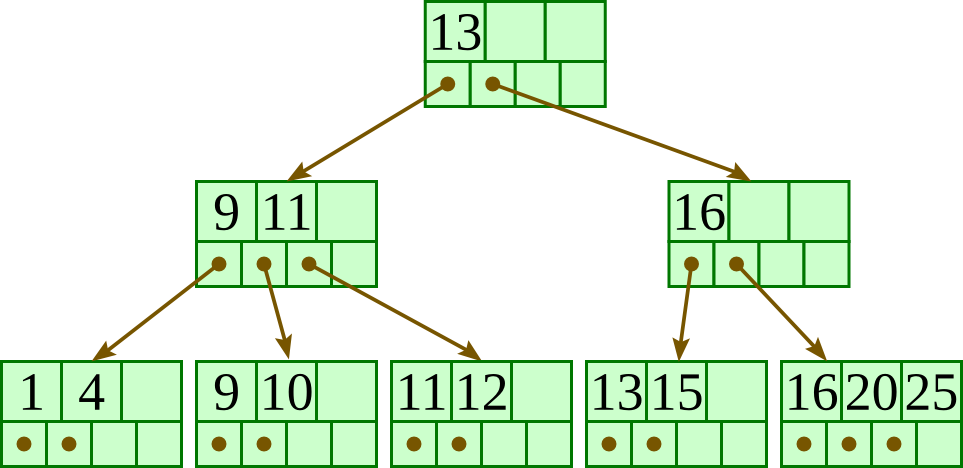
\includegraphics[scale = 0.60]{btree-6.png}
 
Although this seems like a great idea, and the intuitive thing to do would be to index all fields for faster lookups, it is usually not a good idea to do this, because indexes do take up significant space on the disk, and updates on these fields become slower. It is a bad tradeoff to index something that is more likely to be updated than read.Typically, database administrators decide what field(s) to index based on the query workloads and analysis of query logs.

\subsection{NoSQL}
NoSQL databases (of which MapReduce is one) use imperative languages. They might also be called a key-value store. They implement DHT (Distributed hash tables) with CHORD (consistent hashing). An advantage of this is the ability to scale. However, scaling can cause problems with updating indices.

\end{document}
